
%%%%%%%%%%%%%%%%%%%%%%% file typeinst.tex %%%%%%%%%%%%%%%%%%%%%%%%%
%
% This is the LaTeX source for the instructions to authors using
% the LaTeX document class 'llncs.cls' for contributions to
% the Lecture Notes in Computer Sciences series.
% http://www.springer.com/lncs       Springer Heidelberg 2006/05/04
%
% It may be used as a template for your own input - copy it
% to a new file with a new name and use it as the basis
% for your article.
%
% NB: the document class 'llncs' has its own and detailed documentation, see
% ftp://ftp.springer.de/data/pubftp/pub/tex/latex/llncs/latex2e/llncsdoc.pdf
%
%%%%%%%%%%%%%%%%%%%%%%%%%%%%%%%%%%%%%%%%%%%%%%%%%%%%%%%%%%%%%%%%%%%


\documentclass[runningheads,a4paper]{llncs}

\usepackage{amssymb}
\setcounter{tocdepth}{3}
\usepackage{graphicx}
\usepackage{float}
\usepackage{subfigure}

\usepackage{pgfplots}
\usepackage{url}
\usepackage{enumitem}
\usepackage[linesnumbered,ruled]{algorithm2e}
\usepackage[export]{adjustbox}
\usepackage{xspace}
\usepackage{breqn}



\usepackage{url}

\urldef{\mailsb}\path|{tiago.oliveira, bento.francisco, freire.pontes}@academico.ifrn.edu.br|
\urldef{\mailsc}\path|placido.neto@ifrn.edu.br|    
\newcommand{\keywords}[1]{\par\addvspace\baselineskip
\noindent\keywordname\enspace\ignorespaces#1}

\begin{document}

\mainmatter  % start of an individual contribution

% first the title is needed
\title{Can interactivity and guidance be increased by highlighting regions preferences over time?}

% a short form should be given in case it is too long for the running head
\titlerunning{Can interactivity and guidance be increased by highlighting regions preferences over time?}

% the name(s) of the author(s) follow(s) next
%
% NB: Chinese authors should write their first names(s) in front of
% their surnames. This ensures that the names appear correctly in
% the running heads and the author index.
%
\author{Pl\'acido A. Souza Neto \and Tiago Oliveira Lisboa \and \\
Francisco B. Silva Junior \and Felipe F. Pontes }
%
\authorrunning{Souza Neto, Pl\'acido A. \textit{et al.}}
% (feature abused for this document to repeat the title also on left hand pages)

% the affiliations are given next; don't give your e-mail address
% unless you accept that it will be published
\institute{Federal Institute of Rio Grande do Norte (Brazil)\\
\mailsc\\
\mailsb\\
}

%
% NB: a more complex sample for affiliations and the mapping to the
% corresponding authors can be found in the file "llncs.dem"
% (search for the string "\mainmatter" where a contribution starts).
% "llncs.dem" accompanies the document class "llncs.cls".
%

\toctitle{Lecture Notes in Computer Science}
\tocauthor{Authors' Instructions}
\maketitle


\begin{abstract}

Many systems consider space and time information. Discover patterns and provide tendencies in spatiotemporal data applications may improve insights for planning and decision making for smart city solutions. In this way, find spatial and temporal preferences can offer interactive and guidance solutions.  For example,  when users look for a house or hotel to spend a season, they consider one or more regions of their preference. These regions are intrinsic to each user, or user group. However, when navigating the application, the user also considers regions that seem interesting, for different reasons, such as the priority of some tourist spot, restaurants, clubs, security, etc. Thus, capturing region preferences over time can help to guide the user to find better places. In this paper we present a solution to capture region preferences from mouse-tracking and gaze capture. To tackle this challenge, we extend GeoGuide \cite{Omidvar:2017} approach by using ST-DBSCAN\cite{Birant:2007} algorithm to map the region preferences over time. We capture, analyse, generate and save region preferences in order to highlight informations, from any spatiotempotal dataset, that can be useful to the analyst. So, this work aims to answers the question about interactivity and guidance in spatiotemporal approaches.

\keywords{ST-DBSCAN, GeoGuide, mouse-tracking, implicit preferences, regions}
\end{abstract}


\section{Introduction}

%During spatial data analysis, it is often the case that analysts look at some regions of interest but forget to provide an explicit feedback. For instance in Example~\ref{ex:airbnb}, while Liam is focusing on home-stays close to the Eiffel tower, he also looks at farther locations with easy train access. However, he never clicks on those points. 

%We call this latent signal, {\em gaze}. It shown in \cite{fischer1999investigation} that gaze has a strong correlation with ``user attention''. The signal can be captured by tracking eye movements aka saccades~\cite{arapakis2014user}. We employ {\sc ixLabs} gaze tracking\footnote{\it http://www.xlabsgaze.com/} as it only needs a simple web-cam to capture the gaze signal.
 %{\bf Cursor Tracking.} To address privacy issues of web-cam exploitation for gaze tracking, we consider an alternative option of tracking the mouse cursor. It is shown in \cite{arapakis2014understanding} that mouse gestures have a strong correlation with ``user engagement''. Intuitively, a point receives a positive feedback if the cursor moves around it frequently.
 %{\bf Session Time.} In most spatial datasets, there is a profile page dedicated to each point. Examples are restaurant pages in Yelp and lodging pages in Airbnb. We consider the amount of time that the analyst spends in a page as an implicit feedback. For instance, if the analyst spends few minutes in a page for an Indian cuisine restaurant, this counts as positive feedback for this type of restaurants. 

In spatialtemporal data analysis, it is often the case that analysts look at some regions of interest but forget to provide an explicit feedback. To capture user preferences is necessary go beyond filling in attributes and data provided by the user. It is important to understand the user behaviour while using the application to infer about his possible preferences. \cite{Robertson2007}  affirms that temporal change in spatial patterns are increasingly common in geographical analysis. This work explore an approach to the spatialtemporal analysis of polygons that are spatially distinct and experience discrete changes though time. It presents challenges considering changes of regions (polygons) during the time. Works like \cite{Ester:1996} and  \cite{Birant:2007} present solutions for clustering spatialtemporal data. These solutions are relevant to define regions by each cluster that contains important informations for the user. 

It is shown in \cite{Arapakis:2014} that mouse gestures have a strong correlation with ``user engagement''. Intuitively, a point receives a positive feedback if the cursor moves around it frequently. We consider privacy issues by tracking the mouse cursor for each user. We consider the mouse movements an implicit user feedback. In most spatial datasets, there is a profile page dedicated to each point. Examples are restaurant pages in Yelp and lodging pages in Airbnb. In this paper, we consider the amount of time that the user spends in a page as also an implicit feedback. For instance, if the user spends few minutes in a page for an French cuisine restaurant or in a page for an apartment with 2 room and garage, this counts as positive feedback for this type of restaurants.

Let's consider the following example in order to present the ``problem'' to be solve by our proposed approach. 

\begin{example}
\label{ex:benicio}
\textit{Ben\'icio} is planning to live a season in Paris. He decides to rent a home-stay from Airbnb website\footnote{\it http://www.airbnb.com}. As he already know the city, because he has already visited several times before decide to spend a season for study, he is open to any type of lodging, considering some regions of his preferences. He wants to explore his options very carefully. He queries all available locations in Paris with a fair price, although he prefers to live in a more central area of the city, to take better advantage of what Paris can offer. His query results in 3000 locations. As he has no other preferences, an exhaustive investigation needs scanning each location independently which is nearly infeasible. In case he wants to focus on a smaller set of options, it is not clear which subset he needs to look at. While he is looking at primary locations in the list, he shows interest in having ``balcony'' as amenity and being close to Eiffel tower. An ideal system can capture this feedback through mouse-tracking, for instance, in order to short-list a small subset of remaining locations that \textit{Ben\'icio} should consider as high priority based on the regions  which he searched through the mouse movement made on the map of Paris. 
\end{example}


Figure \ref{fig:paris} presents a sequence of maps of Paris, showing a possible  evolution of how can be captured preference regions from \textit{Ben\'icio} search.

Figure \ref{fig:paris0} shows the map before the to use by  \textit{Ben\'icio}. The Figure \ref{fig:paris1} shows 2 regions where the user searched for locations in a time interval $t_1$ (lets consider $n$ seconds as a time interval, and $n < 60$). These two regions intersect each other. The figure \ref{fig:paris2} presents other 2 regions where apartments were also searched at a time interval $t_2$, where $t_1 \prec t_2$. In the same way, figure \ref{fig:paris3}  presents 2 more regions where apartments were searched in a time interval $t_3$, where $t_1 \prec t_2 \prec t_ 3$.

Figures \ref{fig:paris4} and \ref{fig:paris5} highlight the intercessions of all regions. These intercessions show that these regions have been trafficked by the analyst more than once. It can inform a certain preference in these regions. These regions can be captured from mouse tracking or even by gaze techniques. Recognizing highlighted regions can help the analyst to consider one more parameter in the query to identify points in a particular dataset that may be more in line with their needs.

Considering a preference order of regions for \textit{Ben\'icio}, the possible areas for rent would be: (\textit{i}) the intersection of the regions ($r_1 \cap r_2 \cap r_n$), (\textit{i}) the union of the regions minus their intersections (($r_1 \cup r_2 \cup r_n$) - ($r_1 \cap r_2 \cap r_n$)), and finally (\textit{iii}) the entire dataset.

%Figura X apresenta uma sequencia de mapas de Paris descrevendo a evolução de como pode ser capturada as regioes de preferencia de Benício, atraves de captura de movimento do mouse. 

%A figura Y mostra o mapa no momento anterior ao uso pelo analista. A imagem mostra 2 regioes onde o usuario pesquisou por localidades em um intervalo de tempo t1. Essas 2 regioes apresentam interseções entre si. A imagem F apresenta mais 2 regiões onde apartamentos foram procurados em um intervalo de tempo t2, posterior a t1. Da mesma forma a imagem H apresenta mais 2 regiões onde apartamentos foram procurados em um intervalo de tempo t3, posterior a t2. 

%A imagens U e Omostra em destaque as interecesões de todas as regiões. Essas intercesões mostram que essas regiões foram trafegadas pelo analista mais de 1 vês, o que pode informar uma certa preferencia nessas regiões. Essas regiões podem ser capturadas a partir de rastreamento do mouse ou ainda atraves de tecnicas de captura de visão. Reconhecer regiões em destaque, pode auxiliar ao analista a considerar mais um parâmetro na consulta para identificar pontos de um determinado dataset que possam ser mais de acordo com suas necessidades.

\begin{figure} % Inicia o ambiente de figuras
\centering
  \subfigure[Paris map.]{ % Começa a incluir a figura fig1.pdf
   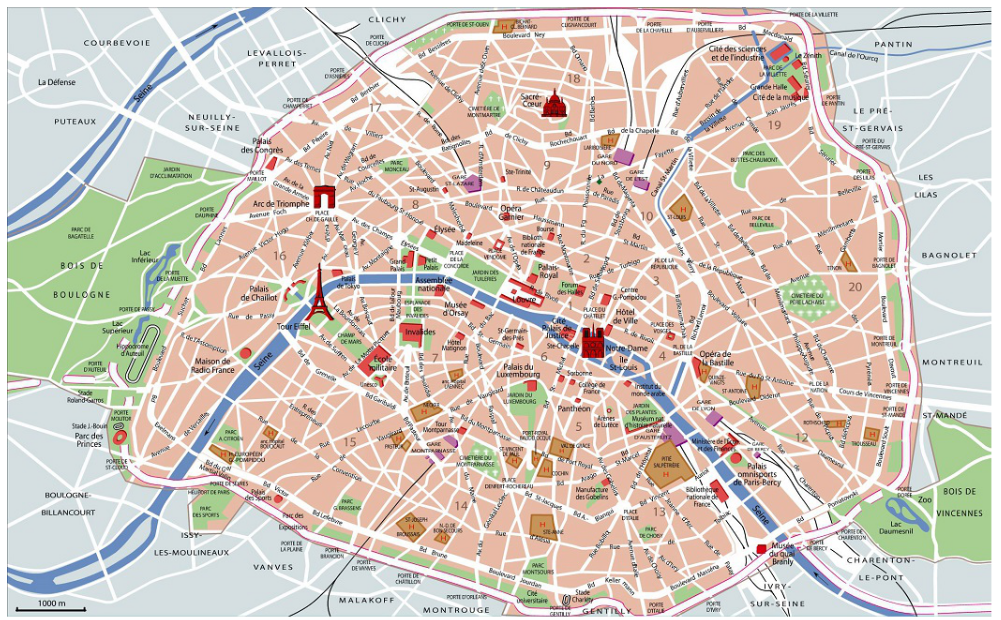
\includegraphics[width=5.8cm]{imgs/adbis2_map0.png}
  \label{fig:paris0} 
  } % Termina de incluir a figura fig1.pdf
  \subfigure[Clusters - time t1.]{ % Começa a incluir a figura fig2.pdf na mesma linha da figura fig1.pdf
    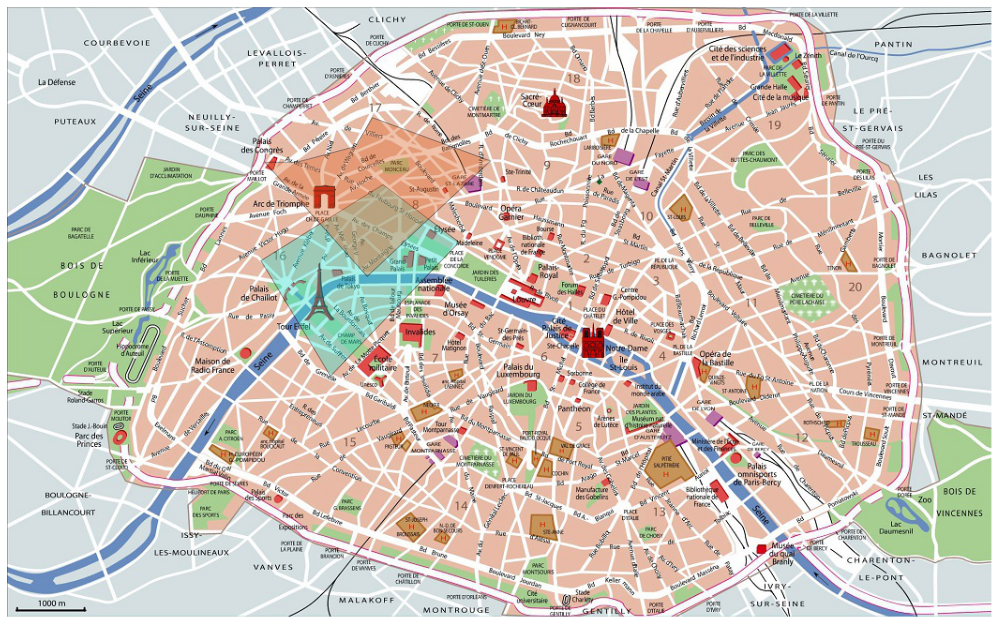
\includegraphics[width=5.8cm]{imgs/adbis2_map1.png}
   \label{fig:paris1}
  } % Termina de incluir a figura fig2.pdf
  \\ % Com esse comando iremos incluir a última figura na próxima linha
  \subfigure[Clusters - time t2.]{ % Começa a incluir a figura fig3.pdf na linha abaixo
    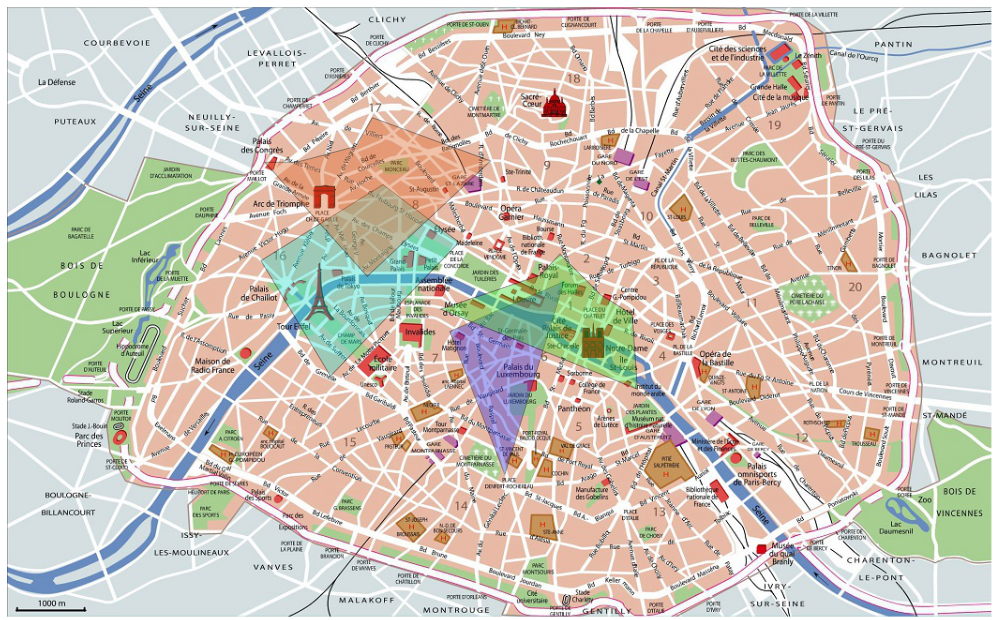
\includegraphics[width=5.8cm]{imgs/adbis2_map2.png}
     \label{fig:paris2} 
  } % Termina de incluir a figura fig3.pdf
   \subfigure[Clusters - time t3.]{ % Começa a incluir a figura fig2.pdf na mesma linha da figura fig1.pdf
    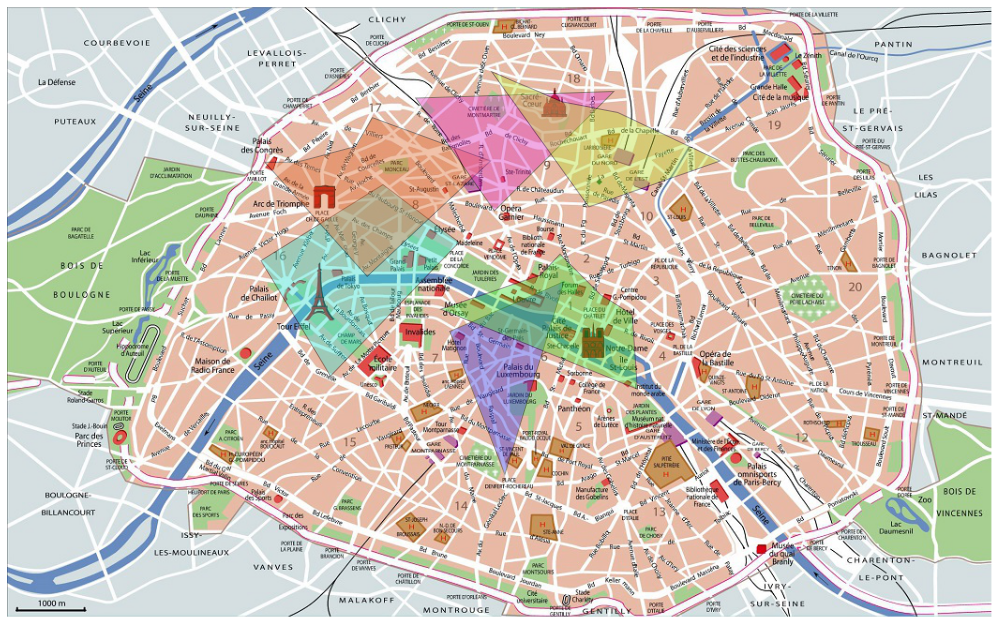
\includegraphics[width=5.8cm]{imgs/adbis2_map3.png}
       \label{fig:paris3} 
  } % Termina de incluir a figura fig2.pdf
  \\ % Com esse comando iremos incluir a última figura na próxima linha
  \subfigure[Intersection of regions.]{ % Começa a incluir a figura fig3.pdf na linha abaixo
    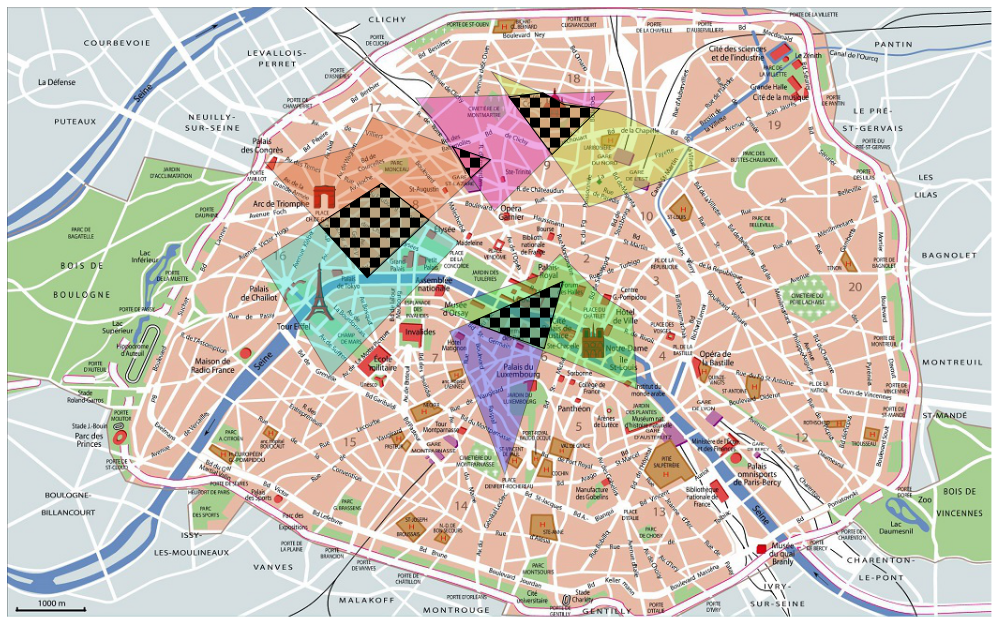
\includegraphics[width=5.8cm]{imgs/adbis2_map4.png}
       \label{fig:paris4} 
  } % Termina de incluir a figura fig3.pdf
   \subfigure[Highlighted regions.]{ % Começa a incluir a figura fig2.pdf na mesma linha da figura fig1.pdf
    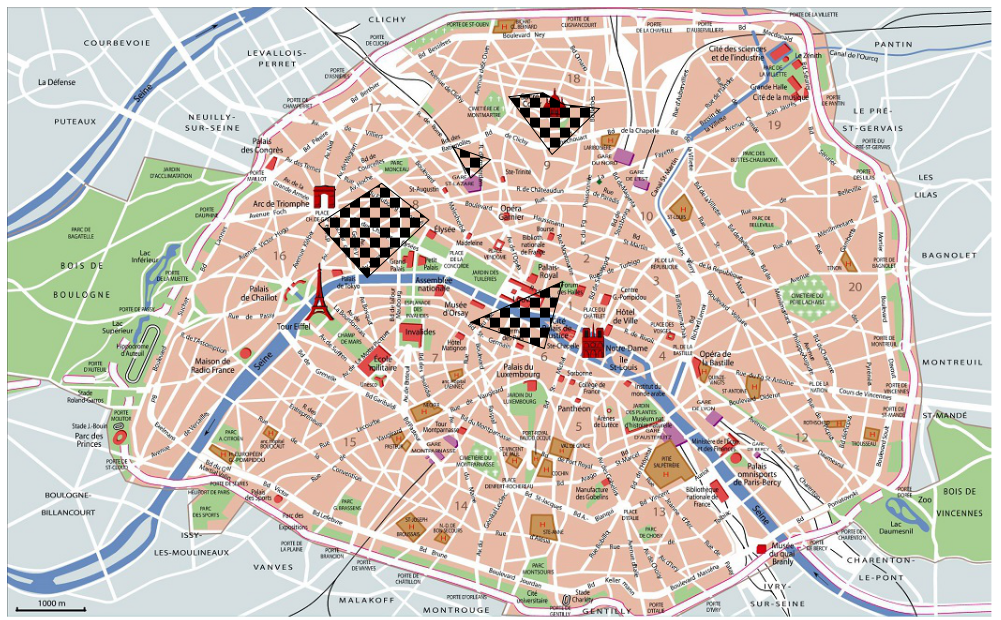
\includegraphics[width=5.8cm]{imgs/adbis2_map5.png}
      \label{fig:paris5} 
  } % Termina de incluir a figura fig2.pdf
  \\ % Com esse comando iremos incluir a última figura na próxima linha
  \caption{Highlighting preference of regions from mouse tracking. }
  \label{fig:paris}
\end{figure} % Fecha o ambiente de figuras

The outline of the paper is as follows: in Section \ref{sec:overpolygons}  we present algorithms to overlap regions over time. Section \ref{sec:scenario}  presents the possible scenarios to run this approach . Section  \ref{sec:experiments}  shows some  experiments and Section \ref{sec:conclusions}  presents some conclusions and future directions. 

\section{Overlapping Polygons by Clustering Spatiotemporal Data}
\label{sec:overpolygons}

This section presents some definitions and concepts in order to describe (\textit{i}) how the polygons are created,(\textit{ii}) in which delay of time the set of polygons are grouped, (\textit{iii})  why and how the polygons are overlapped and  (\textit{iv}) how the regions of preferences over time are defined.

Given a dataset of spatial points and from the mouse tracking movements from the user, our approach generates a set of highlighted regions based on its preferences. Each region is related with a subset highlighted points which are illustrated using visual variables such as size and color intensity. The regions are also highlighted.

\noindent {\bf Data Model.} We consider a spatiotemporal database ${\cal D}$ consisting $\langle {\cal R},  {\cal P}, {\cal A},  \rangle$ where ${\cal R}$ is the set of regions, ${\cal P}$ is the set of
geographical points contained in the regions, and ${\cal A}$ is the set of point attributes.  For each $r \in {\cal R}$,  it contains a set of $p \in {\cal P}$, where $p_1,p_2,...,p_n  \in r \land  r \subset	{\cal P}$. We consider a tuple $\langle lat, lon, t\rangle$ where $lat$, $lon$ and $alt$ denote $p$'s geographical coordinates (latitude and longitude  respectively), and $t$ is the timestamp. The set ${\cal A}_p$ contains attribute-values for $p$ over the schema of ${\cal A}$. 

\begin{algorithm}[t]
	\DontPrintSemicolon
	\KwIn{${\cal R}$ = \{ $r_1, r_2,...,r_n $ \}, $\Delta t \in T$}
	% \KwOut{${\cal S}_p$}
	${ R_p} \gets \emptyset$\;\label{cd:definereturn}
	%$p_{next} \gets get\_next(\mathit{{\cal L}^p})$\;\label{cd:getnext}
	\For{$(r_n \in {\cal R})$}{\label{cd:beginfr}
		\For{$(r_{n+1} \in {\cal R})$}{
			\If{$(r_n \cap r_{n+1} \neq \emptyset \wedge get\_time(r_n) \subseteq t \wedge get\_time(r_{n+1}) \subseteq t $}{\label{cd:if_intersectino}
				${ R_p} \gets  (r_n \cap r_{n+1}) \wedge { R_p}  $\;
			}
		}
	}
	%	$p_{next} \gets get\_next({\cal L}_p)$\;}\label{cd:endwhile}
	\Return{${ R_p}$}\; 
	\caption{{\sc Region Highlighter} Algorithm}
	\label{algo:intersectionAlgo}
\end{algorithm}

The Algorithm \ref{algo:intersectionAlgo} goal is to identify which regions are intersect considering the clusters identified during  the analyst search. The inputs are a set o regions ${\cal R}$  and a time interval $\Delta t$. The list of preferred regions is defined in line \ref{cd:definereturn}. For each region $r_n \in {\cal R}$ (line \ref{cd:beginfr}), the algorithm verifies if there are intersections with  a region $r_{n+1} \in {\cal R}$ (line \ref{cd:if_intersectino}). If there is a intersection and the region time is in the time interval, the intersection $r_n \cap r_{n+1} $ is included in ${ R_p}$.

%For instance, on a bike-sharing dataset, ${\cal A}_p = \langle${\tt female}, {\tt young}, {\tt hybrid-bike}$\rangle$ on the schema ${\cal A} = \langle${\tt gender}, {\tt age}, {\tt type}$\rangle$ denotes that $p$ is associated to a young female cyclist who rides a hybrid bike. The set ${\cal A}$ is domain-dependent and defines the semantics of a spatiotemporal dataset.


\begin{algorithm}[t]
	\DontPrintSemicolon
	\KwIn{$p \in {\cal P}$, $\sigma$, $k$, $tlimit$, $R_{p}$ = \{ $r_{p1}, r_{p2},...,r_{pn} $ \}}
	% \KwOut{${\cal S}_p$}
	${\cal S}_p \gets get\_top\_k(\mathit{{\cal L}^p})$\;\label{cd:gettopk}
	$p_{next} \gets get\_next(\mathit{{\cal L}^p})$\;\label{cd:getnext}
   ${\cal S}_{rp} \gets {\cal S}_p$\;\label{cd:empty_regions}
	\While{$(tlimit$ $not$ $exceeded \wedge relevance(p,p_{next}) \geq \sigma)$}{\label{cd:beginwhile}
		\For{$p_{current} \in {\cal S}_p$}{
			\If{$\mathit{diversity\_improved}({\cal S}_p,{\cal S}_{rp},p_{next},p_{current})$}{\label{cd:betterdiv}
			    \For{$r_{current} \in  R_p$}{
			    		   \If{$p_{current} \in r_{current}$}{ \label{cd:point_in_region}
			    		   		${\cal S}_{rp} \gets \mathit{replace}({\cal S}_{rp},p_{next},p_{current})$\;
				$break$\;
			    		   }
			    }
			
				${\cal S}_p \gets \mathit{replace}({\cal S}_p,p_{next},p_{current})$\;
				$break$\;
			}
		}
		$p_{next} \gets get\_next({\cal L}_p)$\;}\label{cd:endwhile}
	\Return{ ${\cal S}_{rp} \cup {\cal S}_p$
	}\; 
	\caption{{\sc GeoGuide} \cite{Omidvar:2017} +  {\sc Region Highlighter} Algorithm}
	\label{algo:geoh}
\end{algorithm}

Algorithm \ref{algo:geoh} modifies the original {\sc Highlighter} proposal presented in GeoGuide \cite{Omidvar:2017} approach .  
The original begins by retrieving the most relevant points to $p$ by simply retrieving the $k$ highest ranking points in ${\cal L}_p$ (line \ref{cd:gettopk}) and function $get\_next({\cal L}_p)$ (Line \ref{cd:getnext}) returns the next point $p_{next}$ in ${\cal L}_p$ in sequential order. Line \ref{cd:empty_regions} initialize the set of points that will be retrieved by the highlighted regions. At the beginning we consider that there is no preferred regions. So, the sets ${\cal S}_{rp}$ and ${\cal S}_{p}$  are the same. Lines \ref{cd:beginwhile} to \ref{cd:endwhile} iterate over the inverted indexes to determine if other points should be considered to increase diversity while staying within the time limit and not violating the relevance threshold with the selected point. %Since points in ${\cal L}_g$ are sorted on decreasing relevance with $p$, the algorithm can safely stop as soon as the relevance condition is violated (or if the time limit is exceeded).

The algorithm then looks for a candidate point $p_{current} \in {\cal S}_p$ to replace in order to increase diversity. If the candidate point is presented in a region $r$ (line \ref{cd:point_in_region}), the point is included in ${\cal S}_{rp}$, considering the boolean function $\mathit{diversity\_improved}()$ (line \ref{cd:betterdiv}). This function checks if by replacing $p_{current}$ by $p_{next}$ in ${\cal S}_p$, the overall diversity of the new ${\cal S}_p$ increases. If the point is not in the preferred region, it is included into ${\cal S}_p$.

\section{Case Study: A GeoGuide Application}
\label{sec:scenario}

\section{Experiments}
\label{sec:experiments}


\section{Conclusion}
\label{sec:conclusions}





\vspace{-5pt}

\bibliographystyle{abbrv}
\bibliography{main}

\end{document}
